\documentclass[a4paper, 14pt]{extarticle}

% Поля
%--------------------------------------
\usepackage{geometry}
\geometry{a4paper,tmargin=2cm,bmargin=2cm,lmargin=3cm,rmargin=1cm}
%--------------------------------------


%Russian-specific packages
%--------------------------------------
\usepackage[T2A]{fontenc}
\usepackage[utf8]{inputenc} 
\usepackage[english, main=russian]{babel}
%--------------------------------------

\usepackage{textcomp}

% Красная строка
%--------------------------------------
\usepackage{indentfirst}               
%--------------------------------------             


%Graphics
%--------------------------------------
\usepackage{graphicx}
\graphicspath{ {./images/} }
\usepackage{wrapfig}
%--------------------------------------

% Полуторный интервал
%--------------------------------------
\linespread{1.3}                    
%--------------------------------------

%Выравнивание и переносы
%--------------------------------------
% Избавляемся от переполнений
\sloppy
% Запрещаем разрыв страницы после первой строки абзаца
\clubpenalty=10000
% Запрещаем разрыв страницы после последней строки абзаца
\widowpenalty=10000
%--------------------------------------

%Списки
\usepackage{enumitem}

%Подписи
\usepackage{caption} 

%Гиперссылки
\usepackage{hyperref}

\hypersetup {
	unicode=true
}

%Рисунки
%--------------------------------------
\DeclareCaptionLabelSeparator*{emdash}{~--- }
\captionsetup[figure]{labelsep=emdash,font=onehalfspacing,position=bottom}
%--------------------------------------

\usepackage{tempora}
\usepackage{amsmath}
\usepackage{color}
\usepackage{listings}
\lstset{
  belowcaptionskip=1\baselineskip,
  breaklines=true,
  frame=L,
  xleftmargin=\parindent,
  language=Python,
  showstringspaces=false,
  basicstyle=\footnotesize\ttfamily,
  keywordstyle=\bfseries\color{blue},
  commentstyle=\itshape\color{purple},
  identifierstyle=\color{black},
  stringstyle=\color{red},
}

%--------------------------------------
%			НАЧАЛО ДОКУМЕНТА
%--------------------------------------

\begin{document}

%--------------------------------------
%			ТИТУЛЬНЫЙ ЛИСТ
%--------------------------------------
\begin{titlepage}
\thispagestyle{empty}
\newpage


%Шапка титульного листа
%--------------------------------------
\vspace*{-60pt}
\hspace{-65pt}
\begin{minipage}{0.3\textwidth}
\hspace*{-20pt}\centering

\includegraphics[width=\textwidth]{emblem}
\end{minipage}
\begin{minipage}{0.67\textwidth}\small \textbf{
\vspace*{-0.7ex}
\hspace*{-6pt}\centerline{Министерство науки и высшего образования Российской Федерации}
\vspace*{-0.7ex}
\centerline{Федеральное государственное бюджетное образовательное учреждение }
\vspace*{-0.7ex}
\centerline{высшего образования}
\vspace*{-0.7ex}
\centerline{<<Московский государственный технический университет}
\vspace*{-0.7ex}
\centerline{имени Н.Э. Баумана}
\vspace*{-0.7ex}
\centerline{(национальный исследовательский университет)>>}
\vspace*{-0.7ex}
\centerline{(МГТУ им. Н.Э. Баумана)}}
\end{minipage}
%--------------------------------------

%Полосы
%--------------------------------------
\vspace{-25pt}
\hspace{-35pt}\rule{\textwidth}{2.3pt}

\vspace*{-20.3pt}
\hspace{-35pt}\rule{\textwidth}{0.4pt}
%--------------------------------------

\vspace{1.5ex}
\hspace{-35pt} \noindent \small ФАКУЛЬТЕТ\hspace{80pt} <<Информатика и системы управления>>

\vspace*{-16pt}
\hspace{47pt}\rule{0.83\textwidth}{0.4pt}

\vspace{0.5ex}
\hspace{-35pt} \noindent \small КАФЕДРА\hspace{50pt} <<Прикладная Математика и информатика>>

\vspace*{-16pt}
\hspace{30pt}\rule{0.866\textwidth}{0.4pt}
  
\vspace{11em}

\begin{center}
\Large {\bf "Летучка" MQTT} \\ 
\large {\bf по курсу <<Языки и методы программирования>>} \\ 
\large <<Изучение протокола MQTT>>
\end{center}\normalsize

\vspace{8em}


\begin{flushright}
  {Студент группы ИУ9-21Б Хромов М.А.\hspace*{15pt} \\
  \vspace{2ex}
  Преподаватель Посевин Д. П.\hspace*{15pt}}
\end{flushright}

\bigskip

\vfill
 

\begin{center}
\textsl{Москва 2025}
\end{center}
\end{titlepage}
%--------------------------------------
%		КОНЕЦ ТИТУЛЬНОГО ЛИСТА
%--------------------------------------

\renewcommand{\ttdefault}{pcr}

\setlength{\tabcolsep}{3pt}
\newpage
\section{Цель}\label{Sect::task}
\par
Целью лабораторной работы является приобретение навыка разработки на языке JAVA приложения выполняющего запись данных в топик публичного MQTT брокера и приложения чтения данных из топика.
	
 

\section{Задание}\label{Sect::task}
\par
Реализовать на языке JAVA запись и чтение данных в(из) топика в соответствии со своим вариантом, подготовить и прислать отчет, демонстрацию работы программы необходимо записать. 
Вариант 21
\par 
Координаты центров двух окружностей на плоскости и их радиусы.
\par
1- если окружности пересекаются, 0 - в противном случае.

\section {Практическая реализация}
Исходный код программы представлен в листингах~\ref{lst:code1}--~\ref{lst:code5}.
\begin{figure}[!htb]
\begin{lstlisting}[language={},caption={Консольная реализация},label={lst:code1}]
import org.eclipse.paho.client.mqttv3.*;
import org.eclipse.paho.client.mqttv3.persist.MemoryPersistence;
import java.util.Scanner;

public class CirclePublisher {
    public static void main(String[] args) {
        Scanner sc = new Scanner(System.in);
        System.out.println("Введите x1 y1 r1 x2 y2 r2:");
        double x1 = sc.nextDouble();
        double y1 = sc.nextDouble();
        double r1 = sc.nextDouble();
        double x2 = sc.nextDouble();
        double y2 = sc.nextDouble();
        double r2 = sc.nextDouble();

        String pubTopic = "/khrmv/1";
        String broker = "tcp://test.mosquitto.org:1883";
        String clientId = "Khrmv_Publisher";
        MemoryPersistence persistence = new MemoryPersistence();
        String payload = x1 + " " + y1 + " " + r1 + " " + x2 + " " + y2 + " " + r2;

        try {
            MqttClient client = new MqttClient(broker, clientId, persistence);
            MqttConnectOptions connOpts = new MqttConnectOptions();
            connOpts.setCleanSession(true);//stiraempredsessiu

            client.connect(connOpts);//connectkbrokeru
            MqttMessage message = new MqttMessage(payload.getBytes());
            message.setQos(2);//uroven'dostavki
            client.publish(pubTopic, message);
            System.out.println("Отправлено в " + pubTopic + ": " + payload);
            client.disconnect();
        } catch (MqttException e) {
            e.printStackTrace();
        }
    }
}


\end{lstlisting}
\end{figure}
\newpage
\begin{figure}[!htb]
\begin{lstlisting}[language={},caption={Консольная реализация},label={lst:code2}]
import org.eclipse.paho.client.mqttv3.*;
import org.eclipse.paho.client.mqttv3.persist.MemoryPersistence;

public class CircleSubscriber {

    private static final String subTopic = "/khrmv/#";
    private static final String broker = "tcp://test.mosquitto.org:1883";
    private static final String clientId = "Khrmv_Subscriber";
    private static final MemoryPersistence persistence = new MemoryPersistence();

    private static MqttClient client;
    private static MqttConnectOptions connOpts;

    public static void main(String[] args) {
        try {
            client = new MqttClient(broker, clientId, persistence);
            connOpts = new MqttConnectOptions();
            connOpts.setCleanSession(true);

            client.setCallback(new MqttCallback() {

                public void connectionLost(Throwable cause) {
                    System.out.println("Соединение потеряно: " + cause.getMessage());
                    boolean reconnected = false;
                    int attempt = 1;

                    while (!reconnected) {
                        try {
                            System.out.println("Попытка переподключения #" + attempt + "...");
                            client.connect(connOpts);
                            client.subscribe(subTopic);
                            System.out.println("Успешно переподключено.");
                            reconnected = true;
                        } catch (MqttException e) {
                            System.out.println("Не удалось подключиться: " + e.getMessage());
                            try {
                                Thread.sleep(3000);
                            } catch (InterruptedException ie) {
                                ie.printStackTrace();
                            }
                            attempt++;
                        }
                    }
                }

                public void messageArrived(String topic, MqttMessage message) {
                    System.out.println("Получено из " + topic + ": " + message);

                    String[] parts = message.toString().split(" ");
                    if (parts.length != 6) {
                        System.out.println("Ошибка: ожидается 6 значений.");
                        return;
                    }

                    double x1 = Double.parseDouble(parts[0]);
                    double y1 = Double.parseDouble(parts[1]);
                    double r1 = Double.parseDouble(parts[2]);
                    double x2 = Double.parseDouble(parts[3]);
                    double y2 = Double.parseDouble(parts[4]);
                    double r2 = Double.parseDouble(parts[5]);

                    double distance = Math.sqrt(Math.pow(x1 - x2, 2) + Math.pow(y1 - y2, 2));
                    int result = (distance <= r1 + r2 && distance >= Math.abs(r1 - r2)) ? 1 : 0;

                    System.out.println("Результат: " + result);
                }

                public void deliveryComplete(IMqttDeliveryToken token) {}
            });

            client.connect(connOpts);
            client.subscribe(subTopic);
            System.out.println("Слушаю " + subTopic + " ...");

        } catch (MqttException e) {
            e.printStackTrace();
        }
    }
}



\end{lstlisting}
\end{figure}
\newpage
\begin{figure}[!htb]
\begin{lstlisting}[language={},caption={реализация с swing Ui designer},label={lst:code3}]
import javax.swing.*;
import org.eclipse.paho.client.mqttv3.*;
import org.eclipse.paho.client.mqttv3.persist.MemoryPersistence;

public class CirclePublisherForm {
    public JPanel rootPanel;
    public JTextField x1Field;
    public JTextField y1Field;
    public JTextField r1Field;
    public JTextField x2Field;
    public JTextField y2Field;
    public JTextField r2Field;
    public JButton sendButton;

    private final String broker = "tcp://test.mosquitto.org:1883";
    private final String topic = "/khrmv/1";

    public CirclePublisherForm() {
        sendButton.addActionListener(e -> {
            try {
                double x1 = Double.parseDouble(x1Field.getText());
                double y1 = Double.parseDouble(y1Field.getText());
                double r1 = Double.parseDouble(r1Field.getText());
                double x2 = Double.parseDouble(x2Field.getText());
                double y2 = Double.parseDouble(y2Field.getText());
                double r2 = Double.parseDouble(r2Field.getText());

                String payload = x1 + " " + y1 + " " + r1 + " " + x2 + " " + y2 + " " + r2;
                String clientId = "Khrmv_Publisher";

                MqttClient client = new MqttClient(broker, clientId, new MemoryPersistence());
                MqttConnectOptions options = new MqttConnectOptions();
                options.setCleanSession(true);
                client.connect(options);
                client.publish(topic, new MqttMessage(payload.getBytes()));
                client.disconnect();

                JOptionPane.showMessageDialog(null, "Данные отправлены!");

            } catch (Exception ex) {
                JOptionPane.showMessageDialog(null, "Ошибка: " + ex.getMessage());
            }
        });
    }

    public JPanel getRootPanel() {
        return rootPanel;
    }

    public static void main(String[] args) {
        JFrame frame = new JFrame("Circle Publisher");
        frame.setContentPane(new CirclePublisherForm().getRootPanel());
        frame.setDefaultCloseOperation(JFrame.EXIT_ON_CLOSE);
        frame.setSize(350, 300);
        frame.setVisible(true);
    }
}

\end{lstlisting}
\end{figure}
\newpage
\begin{figure}[!htb]
\begin{lstlisting}[language={},caption={реализация с swing Ui designer},label={lst:code4}]
import javax.swing.*;
import org.eclipse.paho.client.mqttv3.*;
import org.eclipse.paho.client.mqttv3.persist.MemoryPersistence;

public class MQTTChatForm {
    public JTextArea chatArea;
    public JTextField inputField;
    public JButton sendButton;
    public JPanel rootPanel;
    public JTextField nicknameField;
    private String nickname = "";

    private static MqttClient client;
    private static MqttConnectOptions connOpts;

    public JPanel getRootPanel() {
        return rootPanel;
    }

    private final String broker = "tcp://test.mosquitto.org:1883";
    private final String topic = "/iu9/mqttchattt";


    public MQTTChatForm() {
        try {
            String clientId = "ChatUser" + System.currentTimeMillis();
            client = new MqttClient(broker, clientId, new MemoryPersistence());
            MqttConnectOptions opts = new MqttConnectOptions();
            opts.setCleanSession(true);
            client.connect(opts);

            chatArea.append("Подключено к чату!\n");

            client.setCallback(new MqttCallback() {
                public void connectionLost(Throwable cause) {
                    chatArea.append("Соединение потеряно\n");
                    boolean reconnected = false;
                    int attempt = 1;

                    while (!reconnected) {
                        try {
                            System.out.println("Попытка переподключения #" + attempt + "...");
                            client.connect(connOpts);
                            client.subscribe(topic);
                            System.out.println("Успешно переподключено.");
                            reconnected = true;
                        } catch (MqttException e) {
                            System.out.println("Не удалось подключиться: " + e.getMessage());
                            try {
                                Thread.sleep(3000);
                            } catch (InterruptedException ie) {
                                ie.printStackTrace();
                            }
                            attempt++;
                        }
                    }
                }

                public void messageArrived(String topic, MqttMessage message) {
                    String messageStr = message.toString();
                    chatArea.append(messageStr + "\n");
                    if (messageStr.equals("WELCOME BACK TO MQTT")) {
                        chatArea.append(nickname + " присоединился к чату.\n");
                    } else if (messageStr.equals("left")) {
                        chatArea.append(nickname + " покинул чат.\n");
                    }
                }

                public void deliveryComplete(IMqttDeliveryToken token) {
                }
            });

            client.subscribe(topic);

            sendButton.addActionListener(e -> {

                String text = inputField.getText().trim();
                if (!text.isEmpty()) {
                    if (nickname.isEmpty()) {
                        nickname = JOptionPane.showInputDialog("Введите ваш никнейм:");
                        if (nickname == null || nickname.trim().isEmpty()) {
                            nickname = "Guest";
                        }


                        try {
                            client.publish(topic, new MqttMessage("WELCOME BACK TO MQTT".getBytes()));
                        } catch (MqttException ex) {
                            ex.printStackTrace();
                        }
                    }


                    try {
                        String fullMessage = nickname + ": " + text;
                        client.publish(topic, new MqttMessage(fullMessage.getBytes()));
                        inputField.setText("");
                    } catch (Exception ex) {
                        chatArea.append("Ошибка отправки\n");
                    }
                }
            });
            inputField.addActionListener(e -> sendButton.doClick());

        } catch (Exception e) {
            JOptionPane.showMessageDialog(null, "Ошибка MQTT: " + e.getMessage());
        }
    }

    public static void main(String[] args) {
        JFrame frame = new JFrame("MQTT Chat");
        MQTTChatForm chatForm = new MQTTChatForm();
        frame.setContentPane(chatForm.getRootPanel());
        frame.setDefaultCloseOperation(JFrame.EXIT_ON_CLOSE);
        frame.setSize(400, 400);
        frame.setVisible(true);
    }
}

\end{lstlisting}
\end{figure}

\newpage

\begin{figure}[!htb]
\begin{lstlisting}[language={},caption={реализация MQTT чата},label={lst:code5}]
import javax.swing.*;
import org.eclipse.paho.client.mqttv3.*;
import org.eclipse.paho.client.mqttv3.persist.MemoryPersistence;

public class MQTTChatForm {
    public JTextArea chatArea;
    public JTextField inputField;
    public JButton sendButton;
    public JPanel rootPanel;
    public JTextField nicknameField;
    private String nickname = "";

    private static MqttClient client;
    private static MqttConnectOptions connOpts;

    public JPanel getRootPanel() {
        return rootPanel;
    }

    private final String broker = "tcp://test.mosquitto.org:1883";
    private final String topic = "/iu9/mqttchattt";


    public MQTTChatForm() {
        try {
            String clientId = "ChatUser" + System.currentTimeMillis();
            client = new MqttClient(broker, clientId, new MemoryPersistence());
            MqttConnectOptions opts = new MqttConnectOptions();
            opts.setCleanSession(true);
            client.connect(opts);

            chatArea.append("Подключено к чату!\n");

            client.setCallback(new MqttCallback() {
                public void connectionLost(Throwable cause) {
                    chatArea.append("Соединение потеряно\n");
                    boolean reconnected = false;
                    int attempt = 1;

                    while (!reconnected) {
                        try {
                            System.out.println("Попытка переподключения #" + attempt + "...");
                            client.connect(connOpts);
                            client.subscribe(topic);
                            System.out.println("Успешно переподключено.");
                            reconnected = true;
                        } catch (MqttException e) {
                            System.out.println("Не удалось подключиться: " + e.getMessage());
                            try {
                                Thread.sleep(3000);
                            } catch (InterruptedException ie) {
                                ie.printStackTrace();
                            }
                            attempt++;
                        }
                    }
                }

                public void messageArrived(String topic, MqttMessage message) {
                    String messageStr = message.toString();
                    chatArea.append(messageStr + "\n");
                    if (messageStr.equals("WELCOME BACK TO MQTT")) {
                        chatArea.append(nickname + " присоединился к чату.\n");
                    } else if (messageStr.equals("left")) {
                        chatArea.append(nickname + " покинул чат.\n");
                    }
                }

                public void deliveryComplete(IMqttDeliveryToken token) {
                }
            });

            client.subscribe(topic);

            sendButton.addActionListener(e -> {

                String text = inputField.getText().trim();
                if (!text.isEmpty()) {
                    if (nickname.isEmpty()) {
                        nickname = JOptionPane.showInputDialog("Введите ваш никнейм:");
                        if (nickname == null || nickname.trim().isEmpty()) {
                            nickname = "Guest";
                        }


                        try {
                            client.publish(topic, new MqttMessage("WELCOME BACK TO MQTT".getBytes()));
                        } catch (MqttException ex) {
                            ex.printStackTrace();
                        }
                    }


                    try {
                        String fullMessage = nickname + ": " + text;
                        client.publish(topic, new MqttMessage(fullMessage.getBytes()));
                        inputField.setText("");
                    } catch (Exception ex) {
                        chatArea.append("Ошибка отправки\n");
                    }
                }
            });
            inputField.addActionListener(e -> sendButton.doClick());

        } catch (Exception e) {
            JOptionPane.showMessageDialog(null, "Ошибка MQTT: " + e.getMessage());
        }
    }

    public static void main(String[] args) {
        JFrame frame = new JFrame("MQTT Chat");
        MQTTChatForm chatForm = new MQTTChatForm();
        frame.setContentPane(chatForm.getRootPanel());
        frame.setDefaultCloseOperation(JFrame.EXIT_ON_CLOSE);
        frame.setSize(400, 400);
        frame.setVisible(true);
    }
}

\end{lstlisting}
\end{figure}
\clearpage
\newpage

\section{Реализация варианта с интерактивной консолью}
\begin{center}
    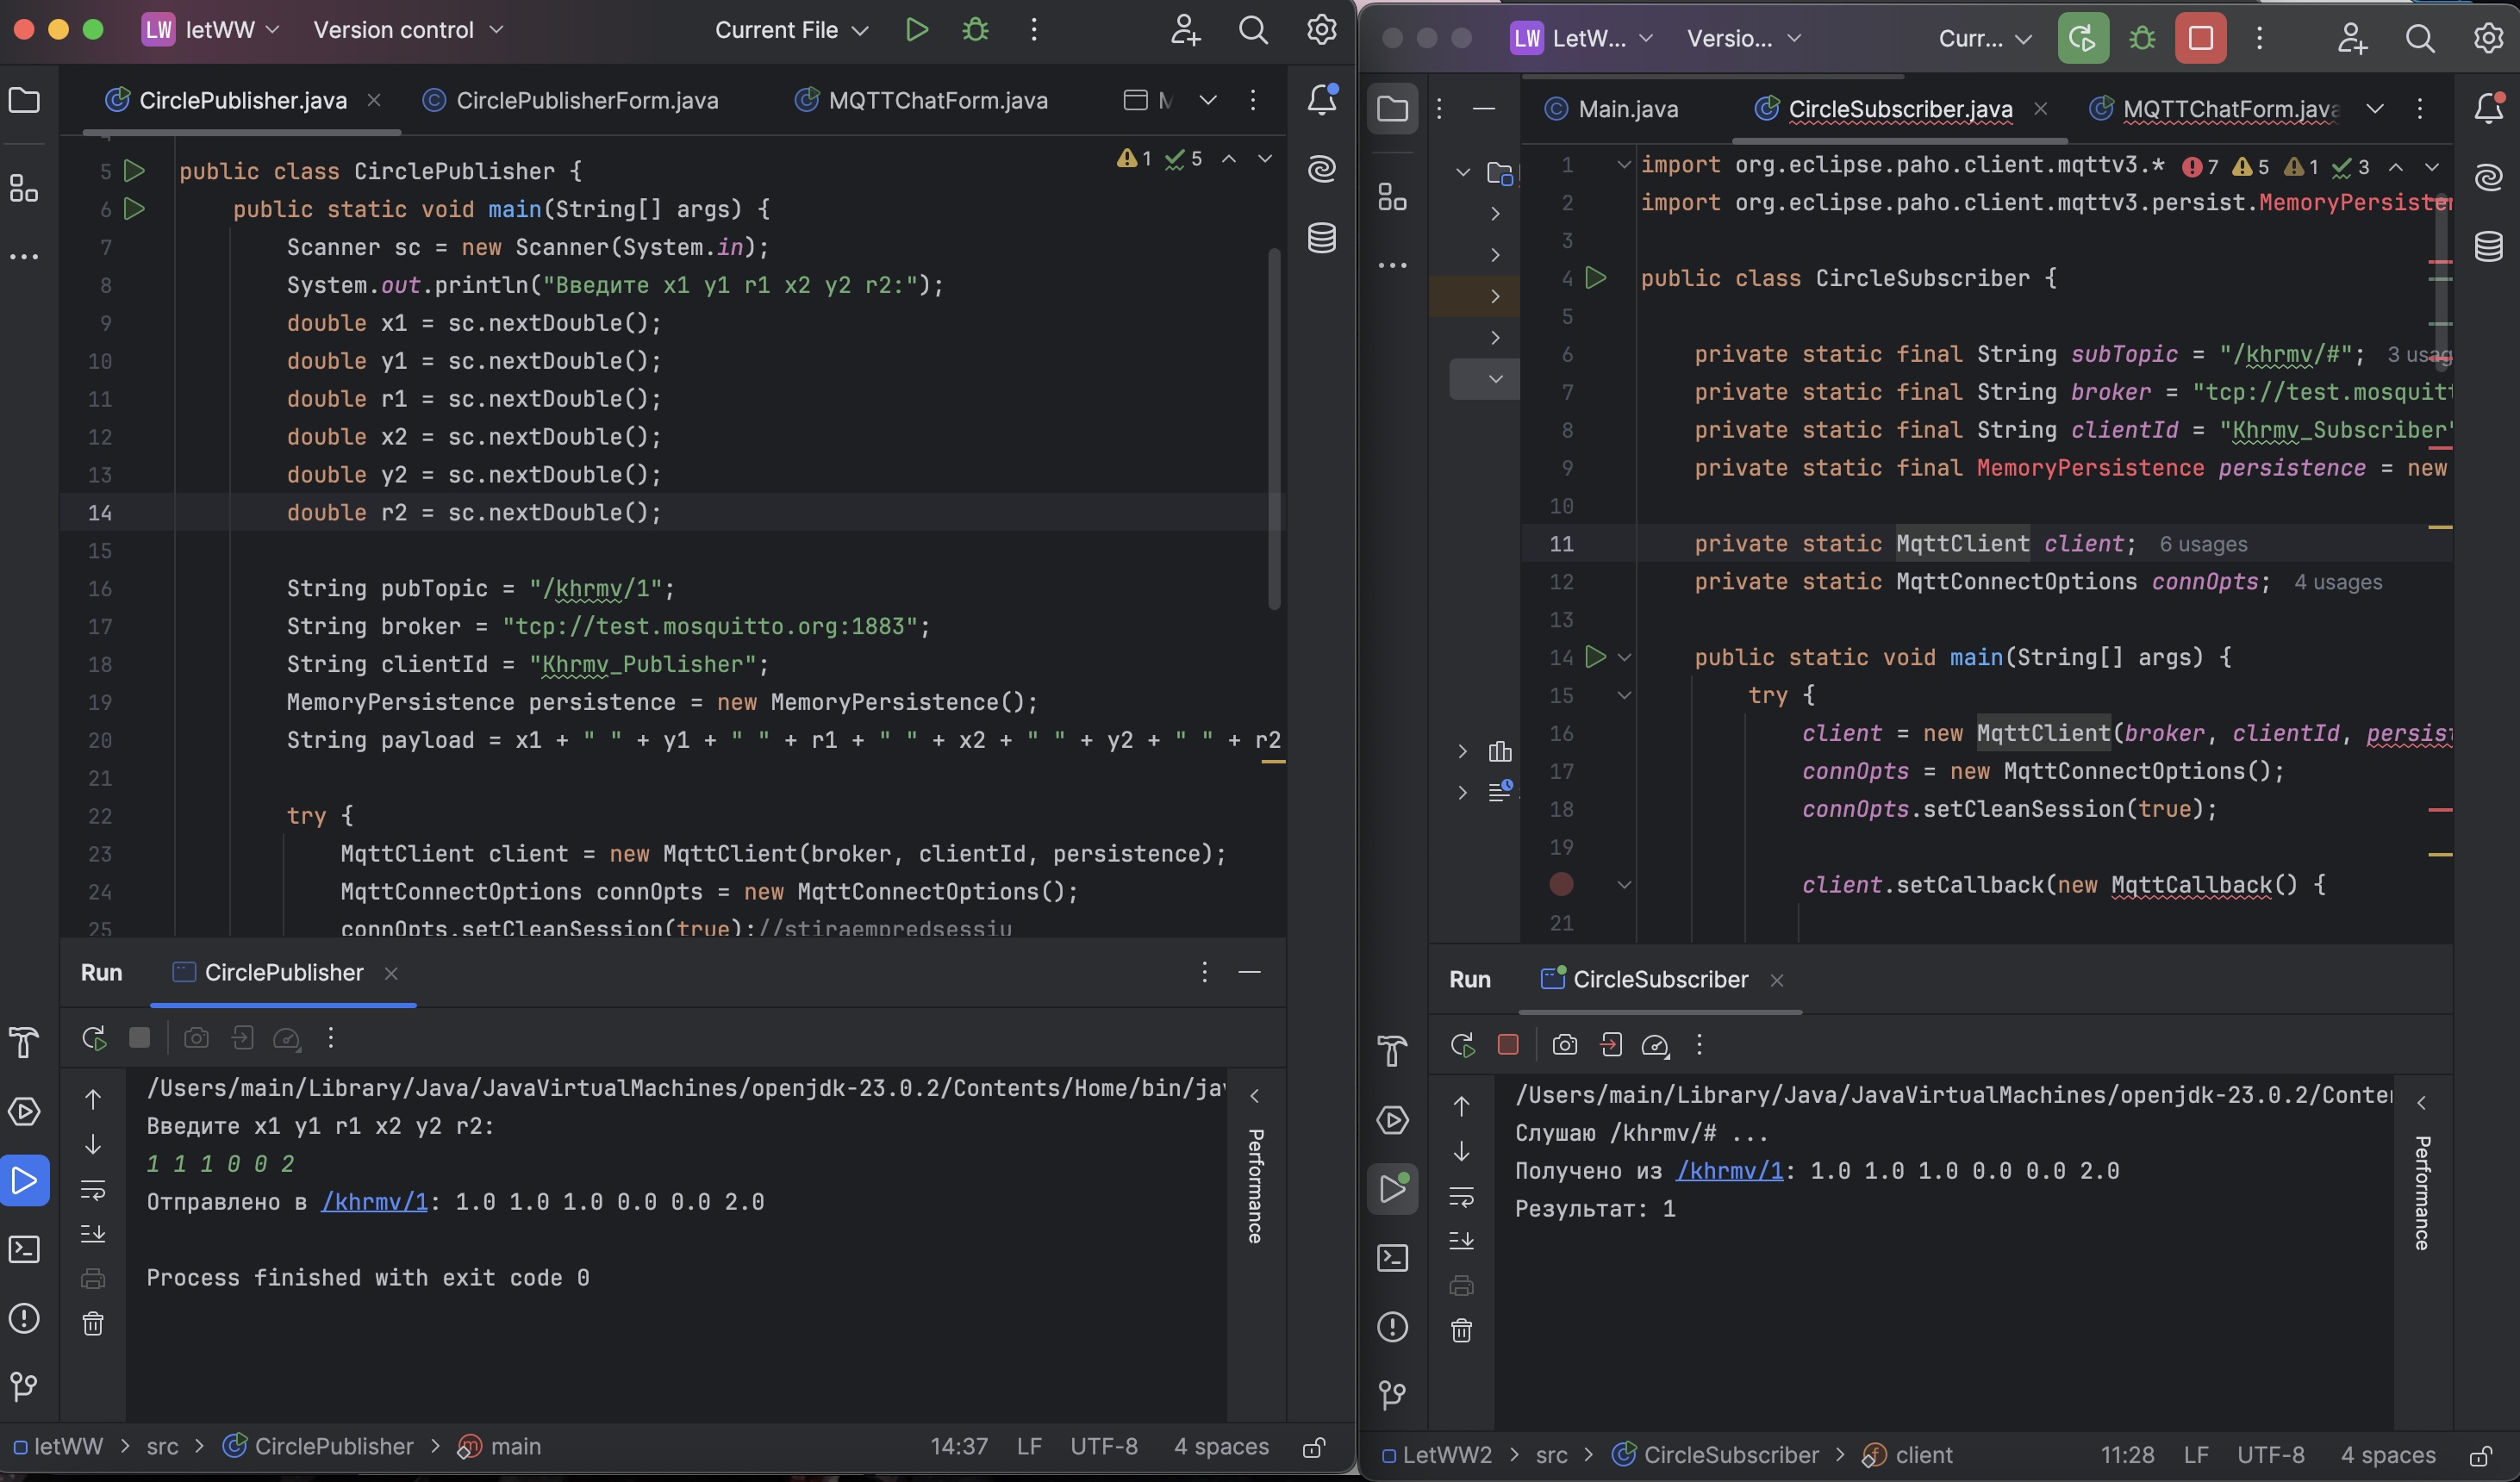
\includegraphics[width=0.8\textwidth]{фото11.jpeg}
    \captionof{figure}{консольная версия}
\end{center}

\begin{center}

    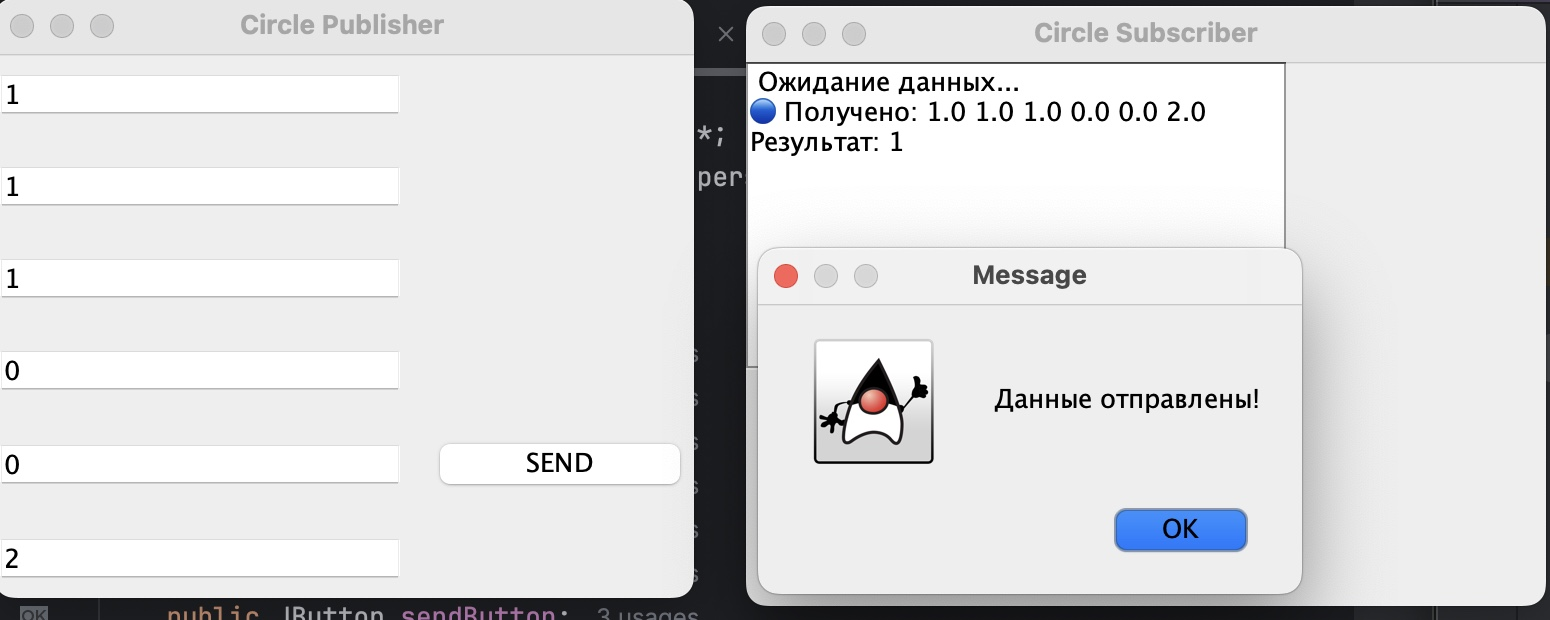
\includegraphics[width=0.8\textwidth]{фото12.jpeg}
    \captionof{figure}{swing версия}
\end{center}
\begin{center}
    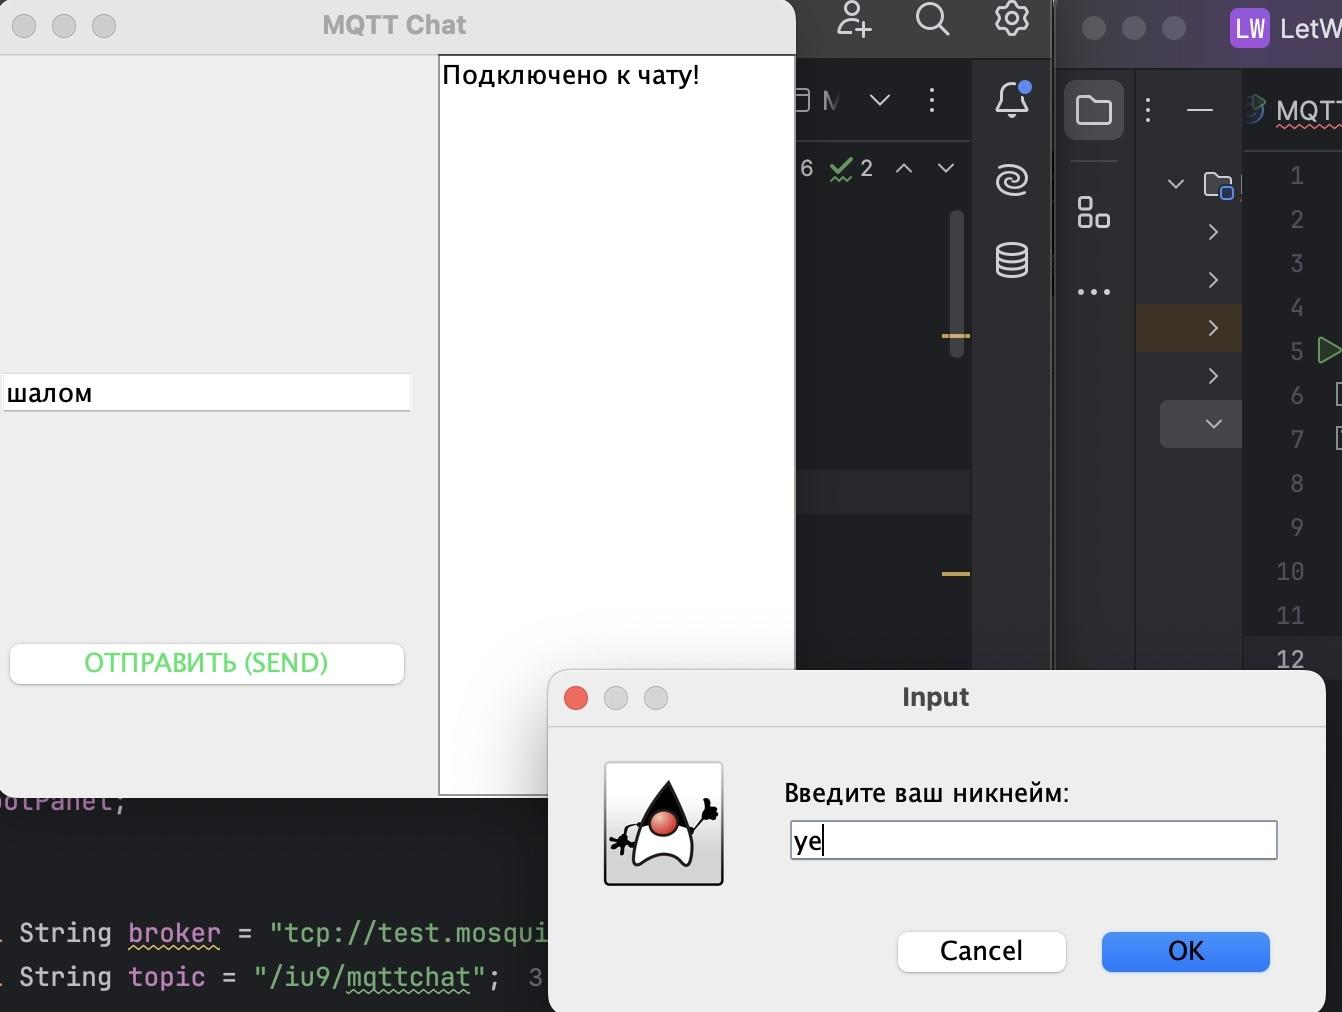
\includegraphics[width=0.8\textwidth]{фото13.jpeg}
    \captionof{figure}{чат}
\end{center}
\newpage
\section{Вывод}
В ходе выполнения данной работы были успешно реализованы три части задания, связанные с технологией MQTT и обработкой геометрических данных.

Первая часть включала разработку двух консольных приложений:

Отправитель (sender) — считывает координаты центров двух окружностей и их радиусы, после чего передает их в MQTT-топик.

Подписчик (subscriber) — получает данные из топика, проверяет условие пересечения окружностей и выводит результат (1 — если пересекаются, 0 — если нет).

Алгоритм проверки пересечения окружностей основывался на сравнении расстояния между центрами с суммой и разностью радиусов, что позволило корректно определять их взаимное расположение.

Во второй части были созданы два GUI-приложения с использованием Swing:

Приложение для ввода данных — предоставляет удобную форму для задания параметров окружностей.

Приложение для вывода результата — отображает, пересекаются ли окружности, на основе полученных данных.

Третья часть представляла собой разработку MQTT-чата с дополнительными функциями:

Поддержка никнеймов — пользователи могут представляться перед отправкой сообщений.

Автоматическое переподключение — при потере соединения чат самостоятельно восстанавливает связь с брокером.

Удобный интерфейс — визуальное разделение сообщений, возможность отслеживания активности участников.

Все задачи выполнены в срок, а в третьей части добавлены улучшения для повышения удобства использования. Работа позволила закрепить навыки работы с MQTT, многопоточностью и графическим интерфейсом на Java.

\end{document}